%%%%%%%%%%%%%%%%%%%%%%%%%%%%%%%%%%%%%%%%%%%%%%%%%%%%%%%%%%%%%%%%%%%%%%
%%  Copyright by Wenliang Du.                                       %%
%%  This work is licensed under the Creative Commons                %%
%%  Attribution-NonCommercial-ShareAlike 4.0 International License. %%
%%  To view a copy of this license, visit                           %%
%%  http://creativecommons.org/licenses/by-nc-sa/4.0/.              %%
%%%%%%%%%%%%%%%%%%%%%%%%%%%%%%%%%%%%%%%%%%%%%%%%%%%%%%%%%%%%%%%%%%%%%%

\newcommand{\devtoolFigs}{../Web_Common/Figs}


% -------------------------------------------
% SUBSECTION
% ------------------------------------------- 
\subsection{Usando \texttt{"HTTP Header Live"} para inspeccionar Encabezados HTTP}
\label{web:sec:httpheaderlive}

La versión de Firefox 60 de nuestra Máquina Virtual de Ubuntu 16.04 no soporta el plugin \texttt{LiveHTTPHeader}, que fue usado en nuestra Máquina Virtual de Ubuntu 12.04.
Dada esta situación, \texttt{"HTTP Header Live"} será usado en su lugar.
Las instrucciones de como habilitar y usar este plugin se muestran en la figura Figure~\ref{web:fig:httpheader} solamente haga click en el ícono marcado en \ding{192}; aparecerá una barra lateral en la izquierda, asegúrese que \texttt{HTTP Header Live} este seleccionada en la posición \ding{193}. Luego haga click en cualquier link dentro de la página, todas los Requests HTTP serán capturados y mostrados dentro de la barra lateral marcada por \ding{194}.
Si hace click en cualquiera Request HTTP, se abrirá un pop-up que mostrará el Request HTTP seleccionado. Desafortunadamente hay un bug en este plugin (que aún se encuentra en desarrollo); no se mostrará nada dentro de este pop-up al menos que ud. cambie su tamaño (Al parecer el evento de re-drawing no es disparado automáticamente cuando se abre el popup, pero cambiando su tamaño ocasiona que este evento sea disparado y en consecuencia se renderize el contenido en pantalla)


\begin{figure}[htb]
\begin{center}
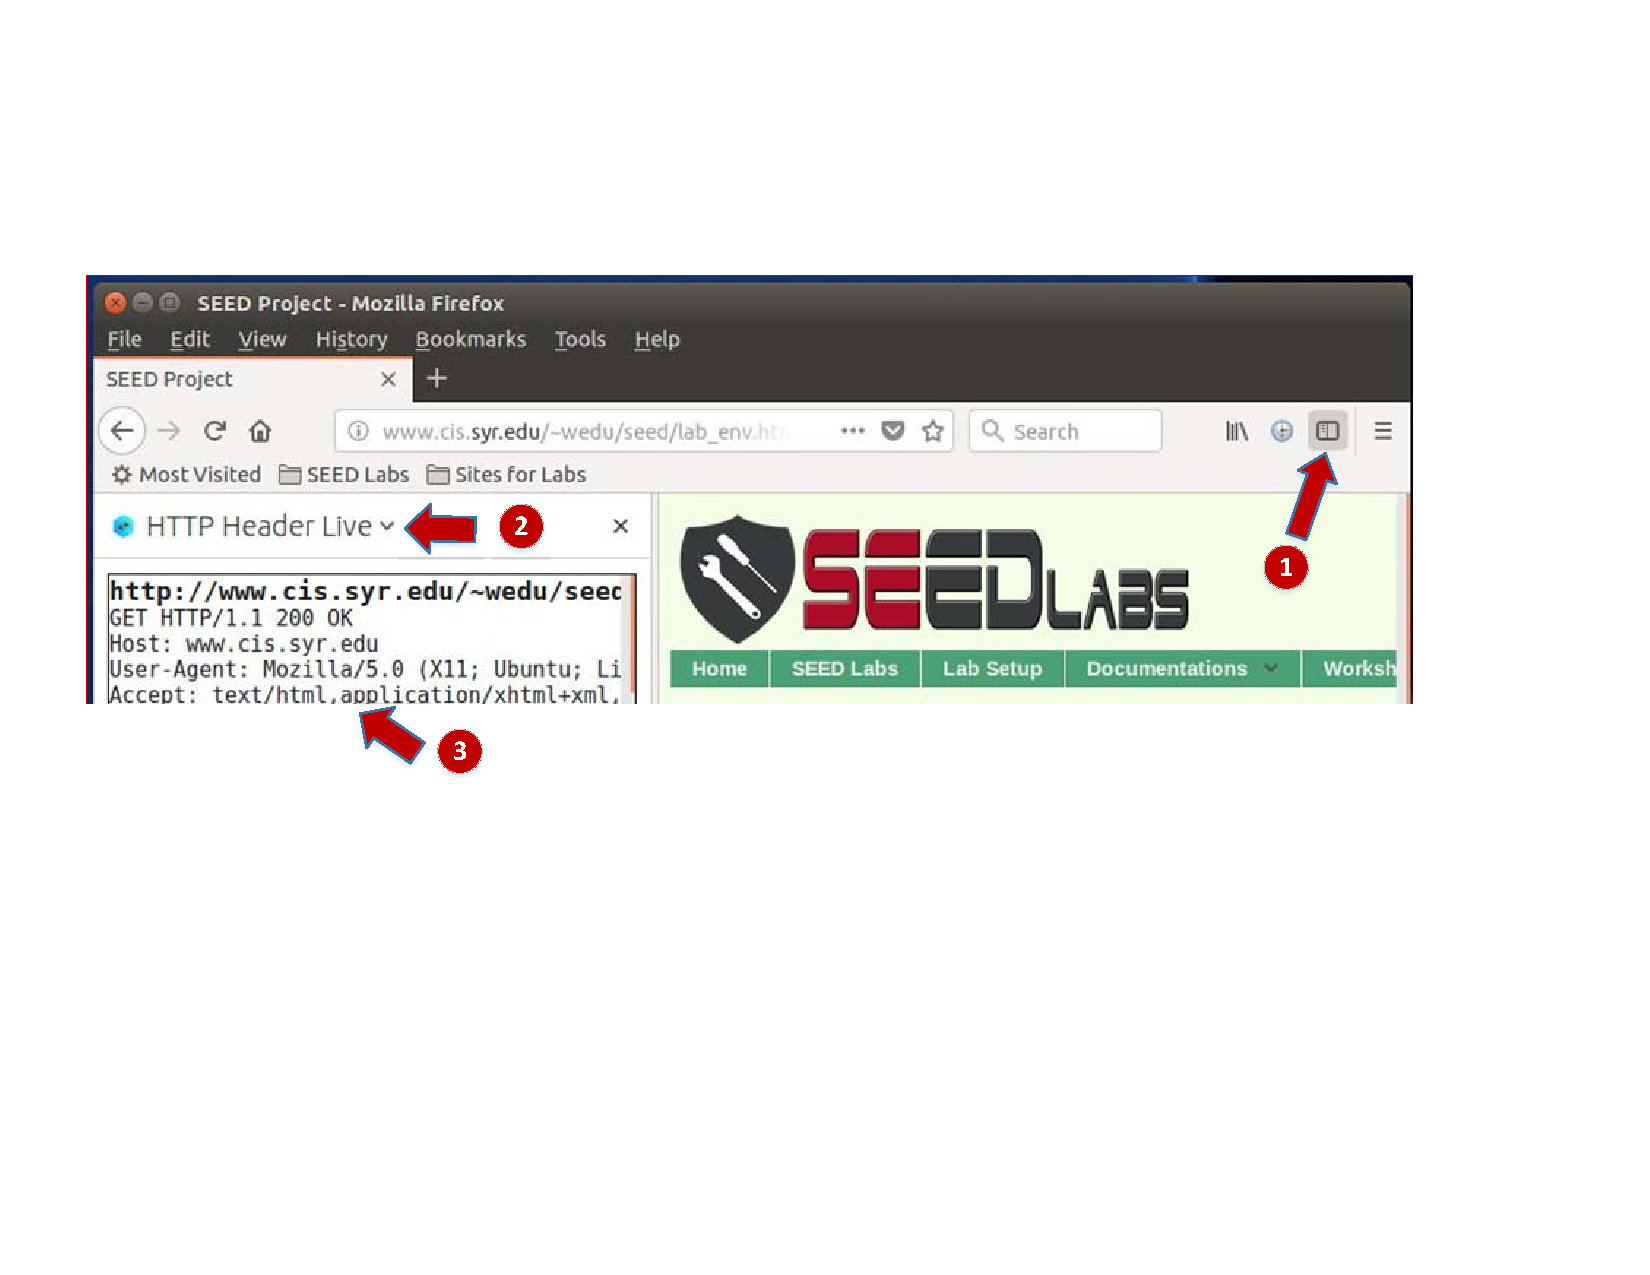
\includegraphics[width=0.85\textwidth]{\devtoolFigs/HTTPHeaderLive.pdf}
\end{center}
\caption{Enable the HTTP Header Live Add-on}
\label{web:fig:httpheader}
\end{figure}




% -------------------------------------------
% SUBSECTION
% ------------------------------------------- 
\subsection{Usando Web Developer Tool para inspeccionar Encabezados HTTP}
\label{web:sec:web_dev_tools}

Existe otra herramienta provista por Firefox que puede ser muy útil para inspeccionoar Encabezados HTTP.
Esta herramienta es la Web Developer Network Tool. En esta sección, vamos a cubrir algunas de las features más importantes de esta herramienta.
La Web Developer Network Tool puede ser habilitada siguiendo estos pasos:

\begin{lstlisting}
Click Firefox's top right menu --> Web Developer --> Network
 or 
Click the "Tools" menu --> Web Developer --> Network 
\end{lstlisting}


We use the user login page in Elgg as an example. 
Figure~\ref{fig:webdevtools_01_request} shows the Network Tool showing the HTTP POST request
that was used for login.

\begin{figure}[htb]
\begin{center}
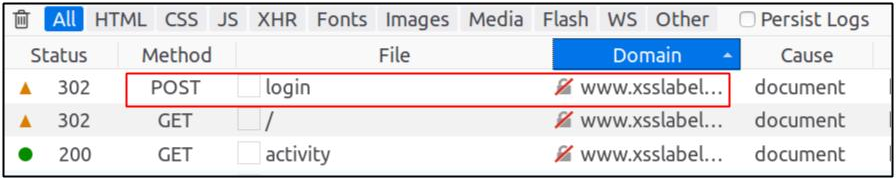
\includegraphics[width=0.8\textwidth]{\devtoolFigs/webdevtools_01_request.png}
\end{center}
\caption{HTTP Request in Web Developer Network Tool}
\label{fig:webdevtools_01_request}
\end{figure}

To further see the details of the request, we can click on a particular HTTP request and the
tool will show the information in two panes (see Figure~\ref{fig:webdevtools_02_two_panes}). 

\begin{figure}[htb]
\begin{center}
	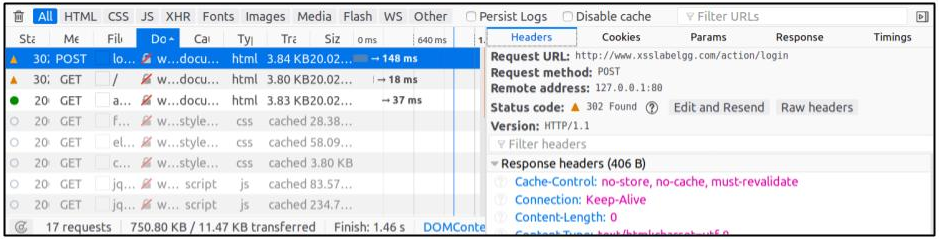
\includegraphics[width=0.95\textwidth]{\devtoolFigs/webdevtools_02_two_panes.png}
\end{center}
\caption{HTTP Request and Request Details in Two Panes}
\label{fig:webdevtools_02_two_panes}
\end{figure}



The details of the selected request will be visible in the right pane.
Figure~\ref{fig:webdevtools_03_post_headers} shows the details of the login request in the
\texttt{Headers} tab (details include URL, request method, and cookie). One can observe both
request and response headers in the right pane. To check the parameters involved in an HTTP
request, we can use the \texttt{Params} tab. Figure~\ref{fig:webdevtools_03_post_params} shows
the parameter sent in the login request to Elgg, including \texttt{username} and
\texttt{password}. The tool can be used to inspect HTTP GET requests in a similar manner to HTTP POST requests.

\begin{figure}[htb]
 \centering
 \subfigure[HTTP Request Headers]{
        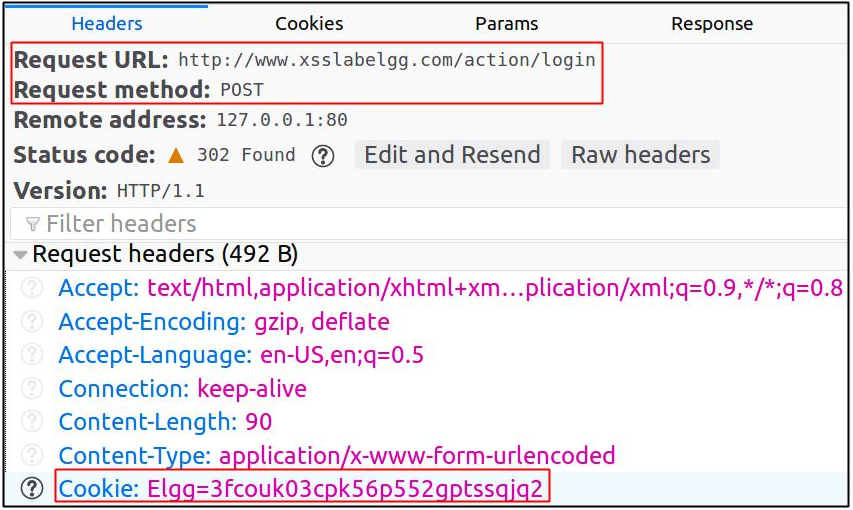
\includegraphics[width=0.6\textwidth]{\devtoolFigs/webdevtools_03-1.png}
        \label{fig:webdevtools_03_post_headers}
 }
 \subfigure[HTTP Request Parameters]{
        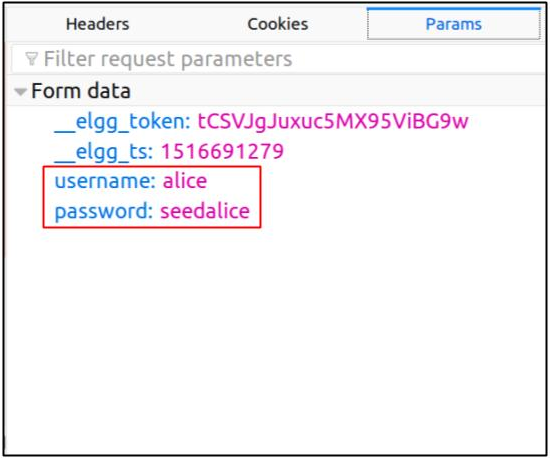
\includegraphics[width=0.35\textwidth]{\devtoolFigs/webdevtools_03-2.png}
        \label{fig:webdevtools_03_post_params}
 }
 \caption{HTTP Headers and Parameters}
\end{figure}


\paragraph{Font Size.} The default font size of Web Developer Tools window is quite small. It
can be increased by focusing click anywhere in the Network Tool window, and then using
\texttt{Ctrl} and \texttt{+} button.


% -------------------------------------------
% SUBSECTION
% -------------------------------------------
\subsection{Debugueando JavaScript}
\label{web:sec:jsdebugging}

We may also need to debug our JavaScript code. Firefox's Developer Tool can also help debug
JavaScript code. It can point us to the precise places where errors occur. The following
instruction shows how to enable this debugging tool:

\begin{lstlisting}
 Click the "Tools" menu --> Web Developer --> Web Console
 or use the Shift+Ctrl+K shortcut.
\end{lstlisting}


Once we are in the web console, click the {\tt JS} tab. Click the downward pointing arrowhead
beside {\tt JS} and ensure there is a check mark beside {\tt Error}. If you are also interested
in Warning messages, click {\tt Warning}. See Figure~\ref{devtool:fig:errocheckmark}.


\begin{figure}[htb]
\begin{center}
  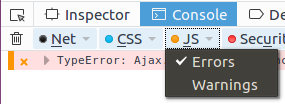
\includegraphics[width=0.4\textwidth]{\devtoolFigs/errorCheckMark.png}
\end{center}
\caption{Debugging JavaScript Code (1)}
\label{devtool:fig:errocheckmark}
\end{figure}
 

If there are any errors in the code, a message will display in the console. The line that
caused the error appears on the right side of the error message in the console. Click on the
line number and you will be taken to the exact place that has the error.
See Figure~\ref{devtool:fig:console}.


\begin{figure}[htb]
\begin{center}
  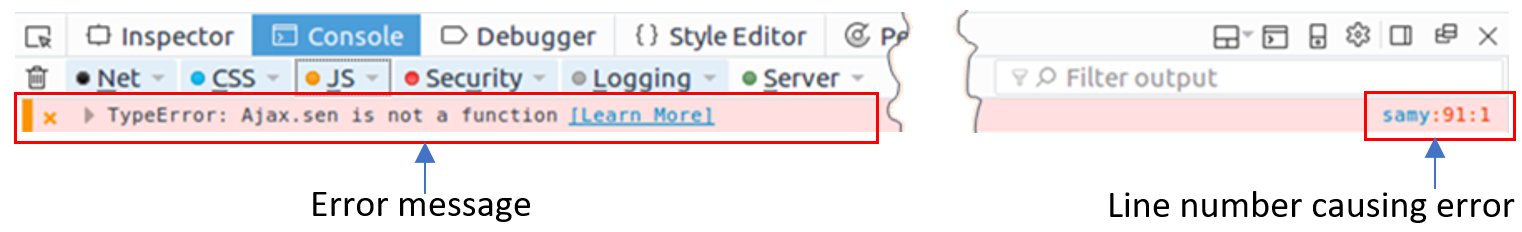
\includegraphics[width=1.0\textwidth]{\devtoolFigs/consoleError2.png}
\end{center}
\caption{Debugging JavaScript Code (2)}
\label{devtool:fig:console}
\end{figure}
 




 
